\newpage
\section{Decider for ``Translated cyclers''}\label{sec:translated-cyclers}

\begin{figure}[h!]
  \centering
  % 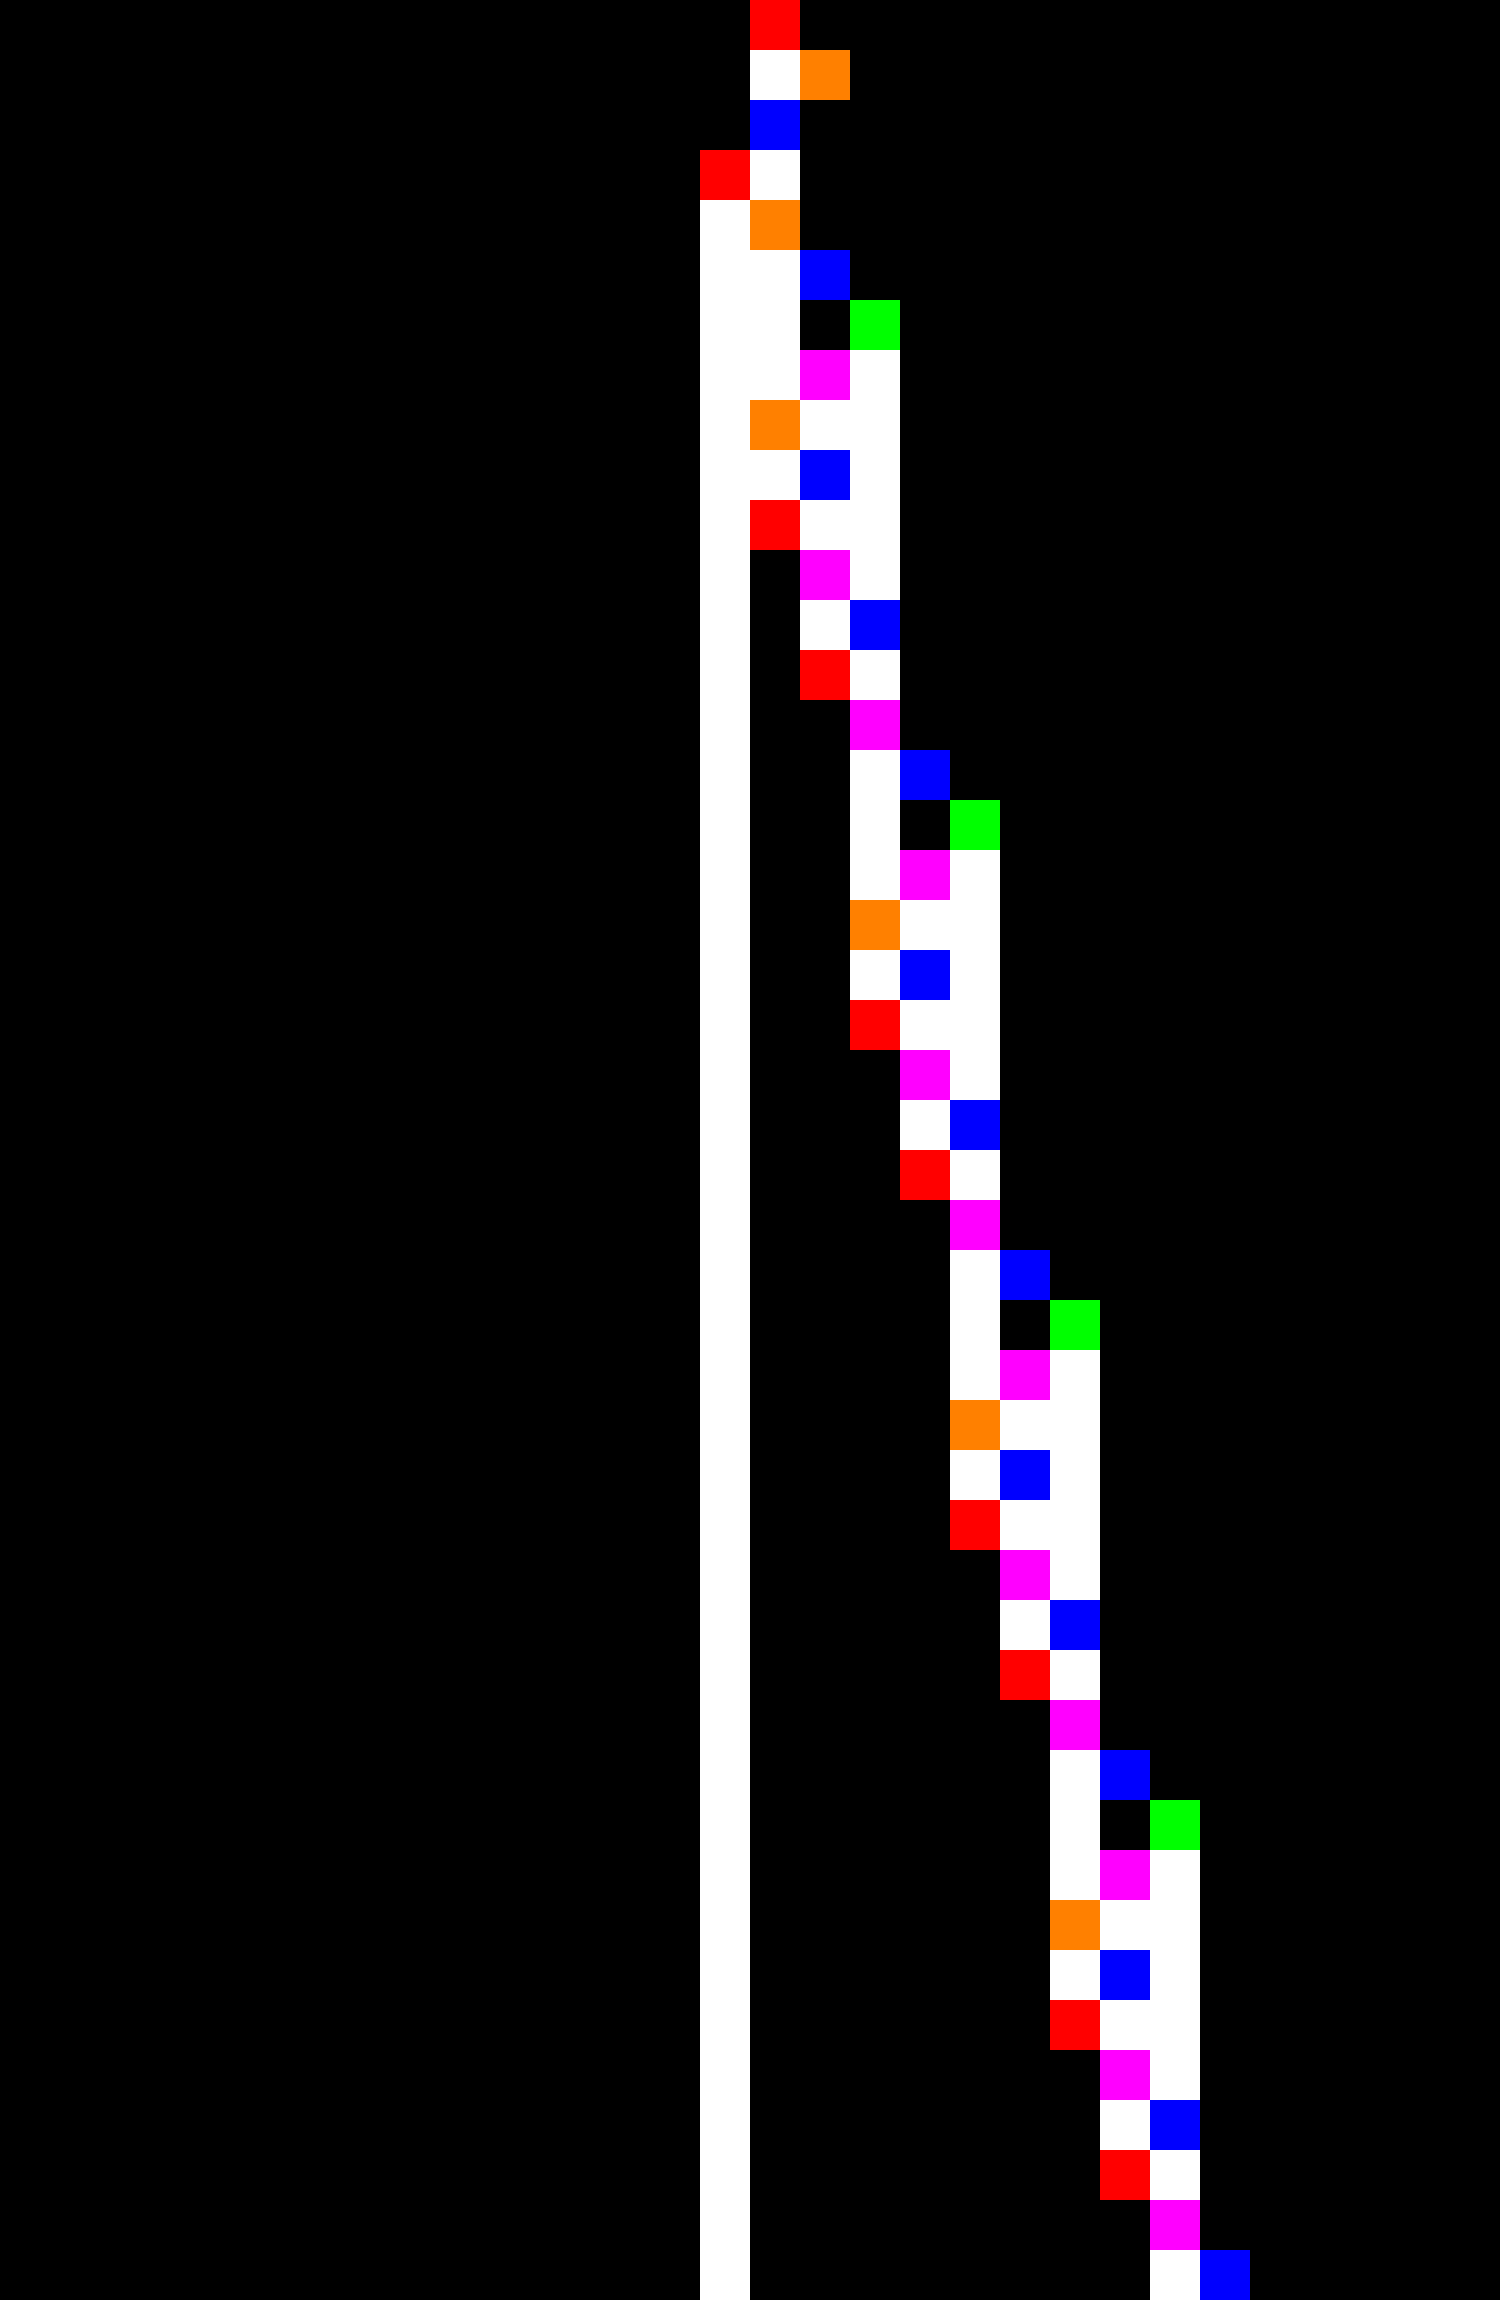
\includegraphics[width=0.5\textwidth]{space-time-diagrams/translated_cycler_44394115.pdf}
  % \hspace{2ex}
  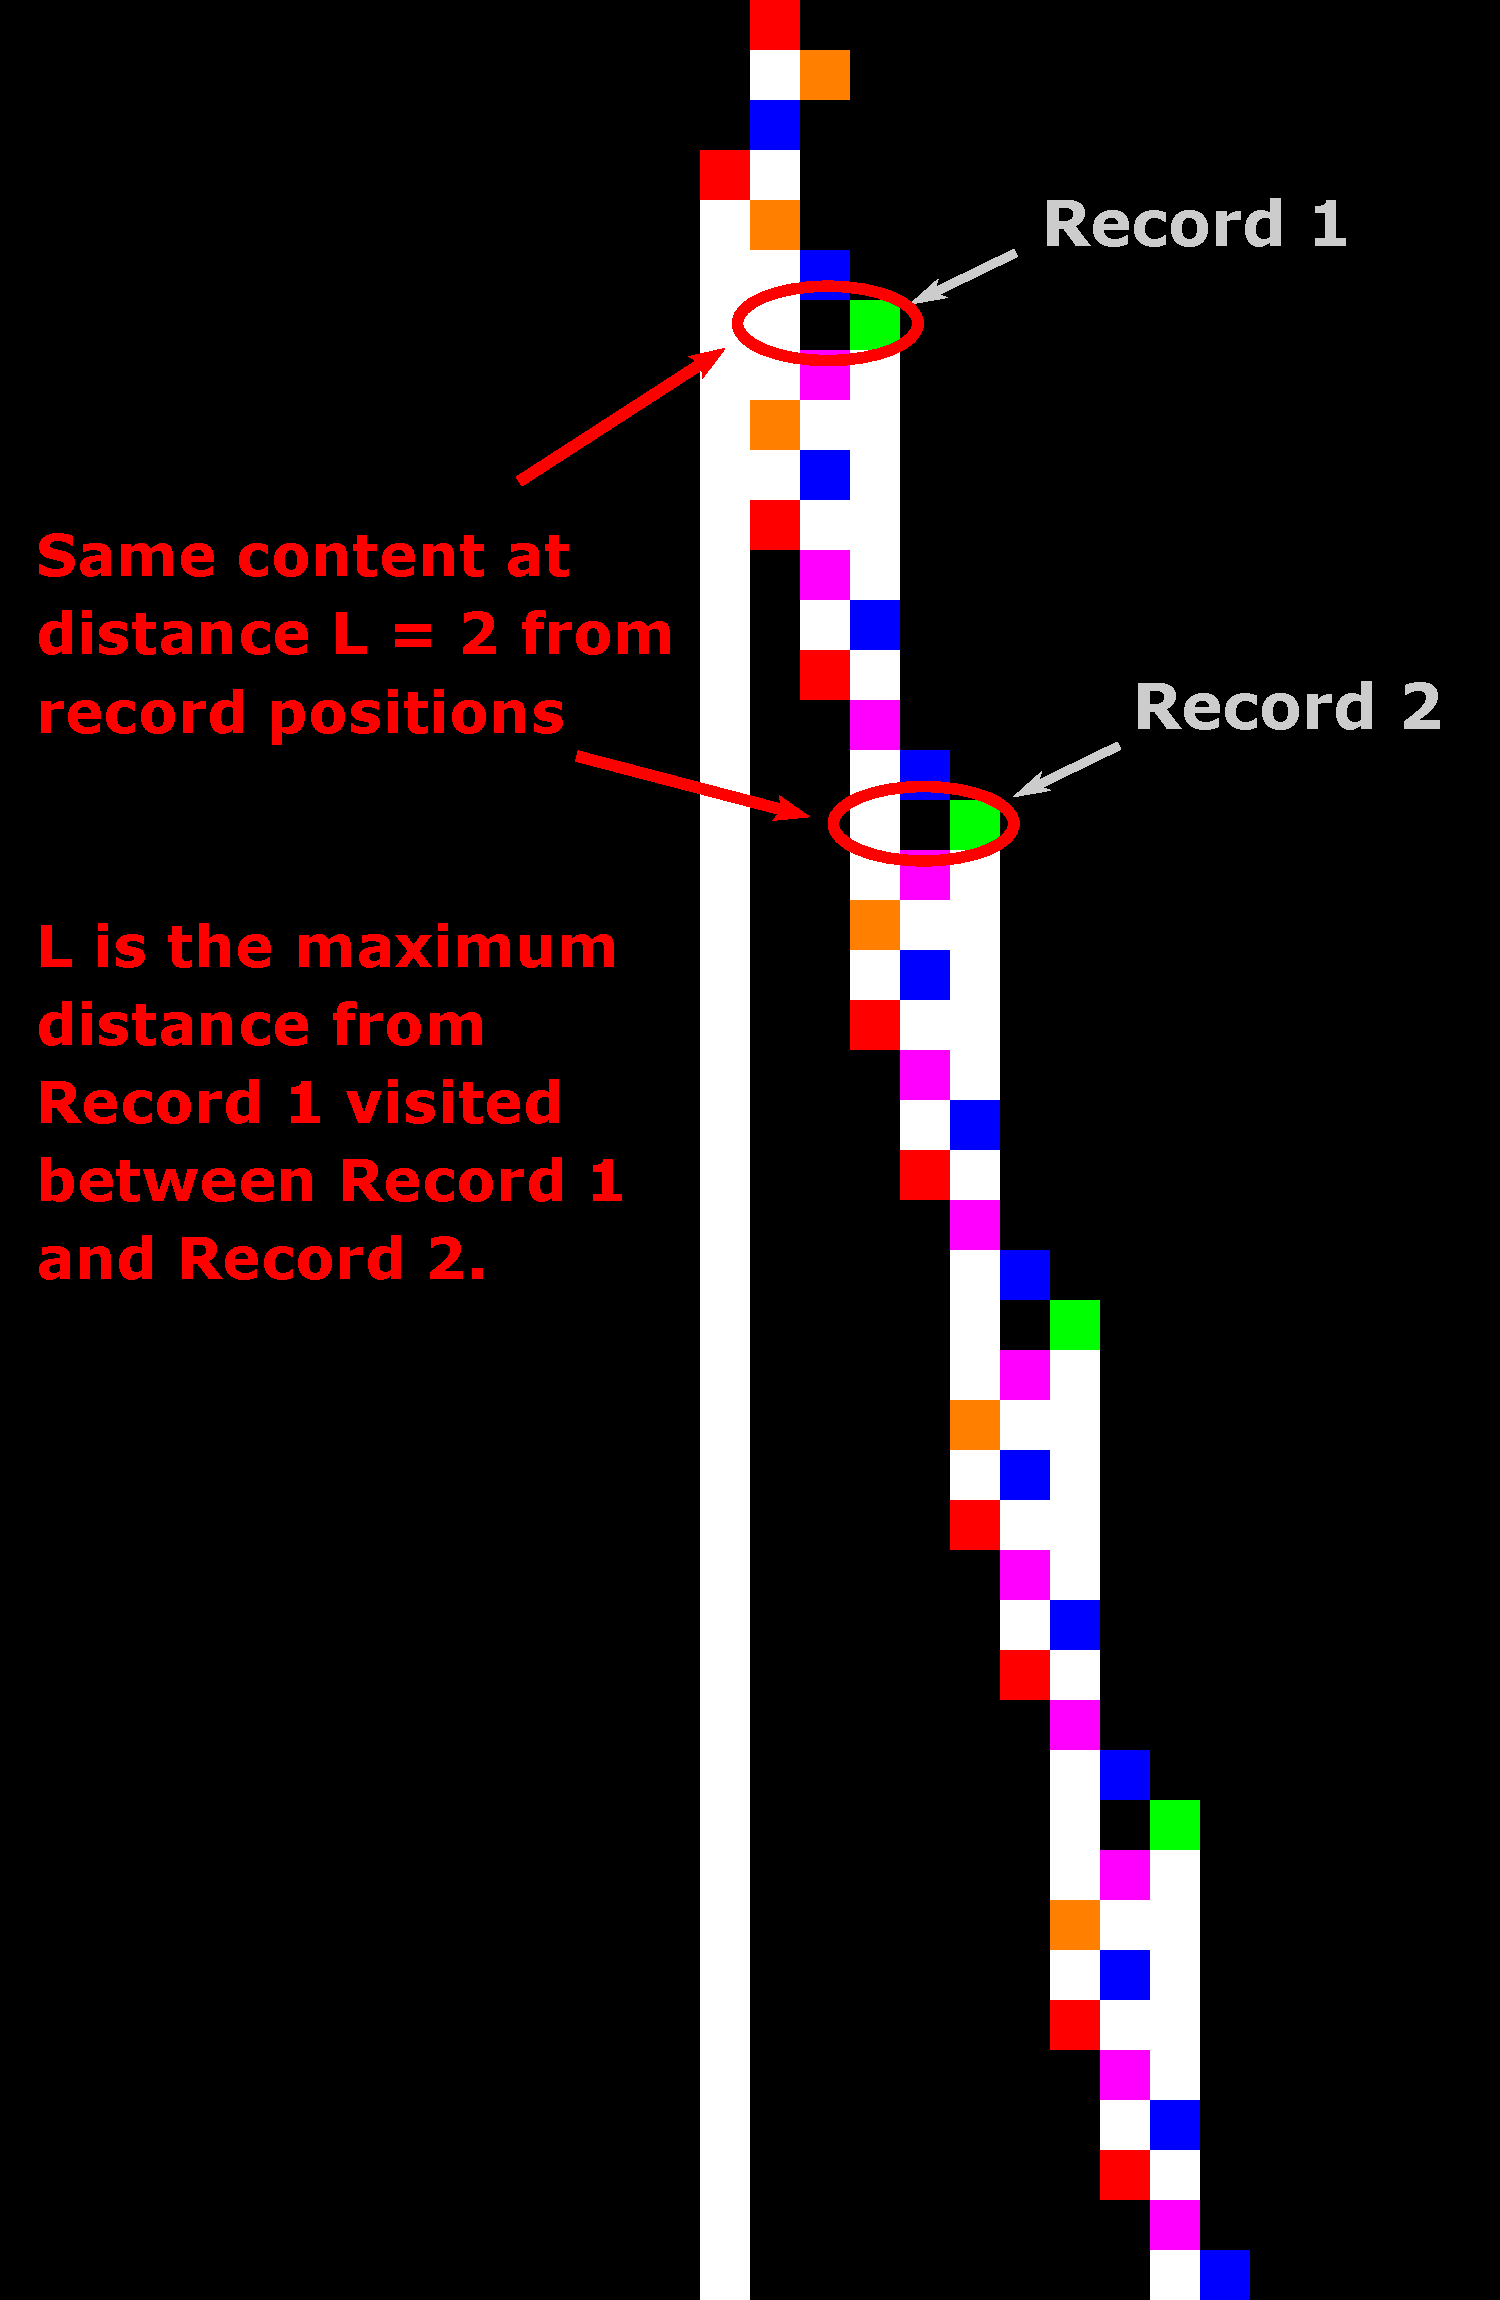
\includegraphics[width=0.54\textwidth]{space-time-diagrams/translated_cycler_44394115_annotated.pdf}

  \caption{Example ``Translated cycler'': 45-step space-time diagram of bbchallenge's machine \#44,394,115. See \url{https://bbchallenge.org/44394115}. The same bounded pattern is being translated to the right for ever. The text annotations illustrate the main idea for recognising ``Translated Cyclers'': find two configurations that break a record (i.e. visit a memory cell that was never visited before) in the same state (here state \textcolor{colorD}{D}) such that the content of the memory tape at distance L from the record positions is the same in both record configurations. Distance L is defined as being the maximum distance to record position 1 that was visited between the configuration of record 1 and record 2.}\label{fig:translated-cyclers}
  \end{figure}
  
The goal of this decider is to recognise Turing machines that translate a bounded pattern for ever. We call such machines ``Translated cyclers''. They are close to ``Cyclers'' (Section~\ref{sec:cyclers}) in the sense that they are only repeating a pattern but there is added complexity as they are able to translate the pattern in space at the same time, hence the decider for Cyclers cannot directly apply here.

The main idea for this decider is illustrated in Figure~\ref{fig:translated-cyclers} which gives the space-time diagram of a ``Translated cycler': bbchallenge's machine \#44,394,115 (c.f. \url{https://bbchallenge.org/44394115}). The idea is to find two configurations that break a record (i.e. visit a memory cell that was never visited before) in the same state (here state \textcolor{colorD}{D}) such that the content of the memory tape at distance L from the record positions is the same in both record configurations. Distance L is defined as being the maximum distance to record position 1 that was visited between the configuration of record 1 and record 2. In those conditions, we can prove that the machine will never halt.

The translated cycler of Figure~\ref{fig:translated-cyclers} features a relatively simple repeating pattern and transient pattern (pattern occurring before the repeating patterns starts). These can get significantly more complex, bbchallenge's machine \#59,090,563 is an example see Figure~\ref{fig:translated-cyclers-more} and \url{https://bbchallenge.org/59090563}. The method for detecting the behavior is the same but more resources are needed.


\begin{figure}
\centering
% 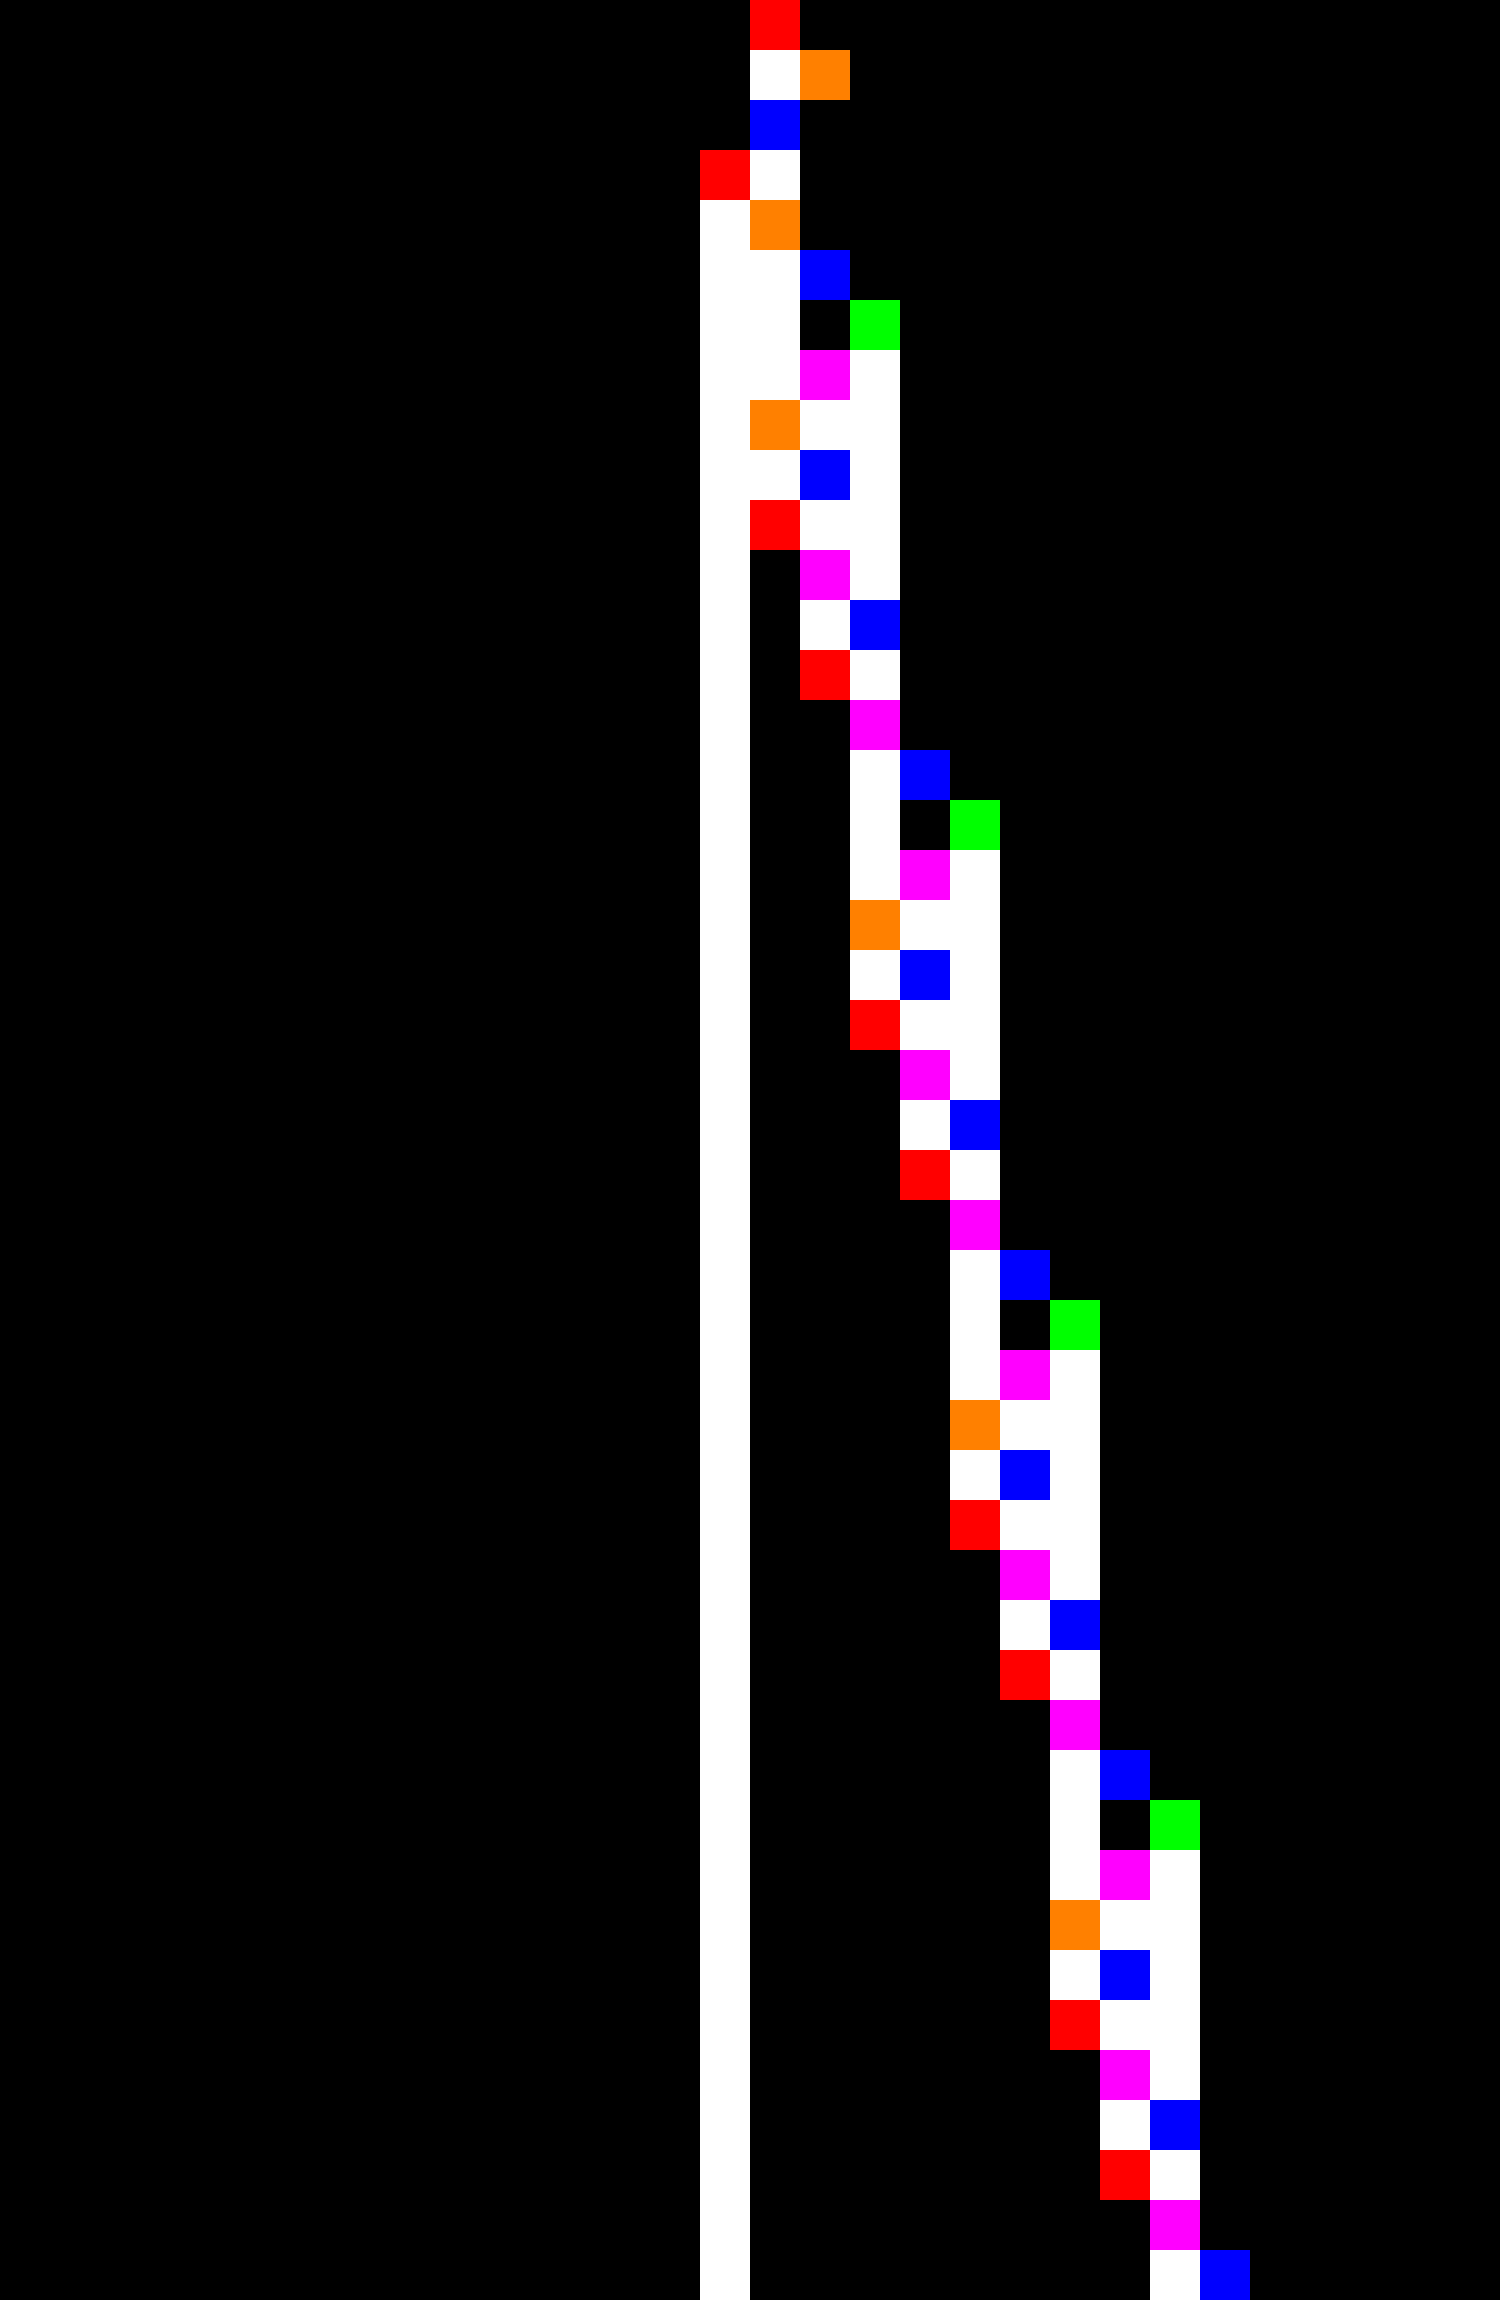
\includegraphics[width=0.5\textwidth]{space-time-diagrams/translated_cycler_44394115.pdf}
% \hspace{2ex}
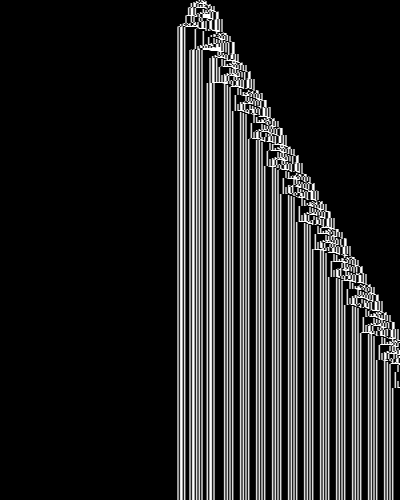
\includegraphics[width=0.7\textwidth]{space-time-diagrams/translated_cycler_59090563.png}

\caption{More complex ``Translated cycler'': 10,000-step space-time diagram (no state colours) of bbchallenge's machine \#59,090,563. See \url{https://bbchallenge.org/59090563}.}\label{fig:translated-cyclers-more}
\end{figure}


\subsection{Pseudocode}

We assume that we are given a Turing Machine type \textbf{TM} that encodes the transition table of a machine as well as a procedure \textbf{TuringMachineStep}(machine,configuration) which computes the next configuration of a Turing machine from the given configuration or \textbf{nil} if the machine halts at that step.

One minor complication of the technique described above is that one has to track record-breaking configurations on both sides of the tape: a configuration can break a record on the right or on the left. Also, in order to compute distance $L$ (see above or Definition~\ref{def:distL}) it is useful to add to memory cells the information of the last time step at which it was visited.

We also assume that we are given a routine {\sc get-extreme-position}(tape,sideOfTape) which gives us the rightmost or leftmost position of the given tape (well defined as we always manipulate finite tapes).

\begin{algorithm}
        \caption{{\sc decider-translated-cylers}}\label{alg:translated-cyclers}

        \begin{algorithmic}[1]
          \State \textbf{const int} RIGHT, LEFT = 0, 1 
          \State \textbf{struct} ValueAndLastTimeVisited \{
            \State \tabi\textbf{int} value
            \State \tabi\textbf{int} lastTimeVisited
            

            \State \}
                \State \textbf{struct} Configuration \{
                \State \tabi\textbf{int} state
                \State \tabi\textbf{int} headPosition
                \State \tabi\textbf{int $\boldsymbol{\to}$ ValueAndLastTimeVisited} tape
                \State \}
                \State 
                

                \Procedure{\textbf{bool} {\sc decider-translated-cylers}}{\textbf{TM} machine,\textbf{int} timeLimit}
                \State \textbf{Configuration} currConfiguration = \{.state = 0,$\,$.headPosition = 0,$\,$ .tape = \{0:\{.value = 0, .lastTimeVisited = 0\}\}\}
                \State // 0: right records, 1: left records
                \State \textbf{List$\boldsymbol{<}$Configuration$\boldsymbol{>}$} 
                recordBreakingConfigurations[2] = [[],[]] 
                \State \textbf{int} extremePositions[2] = [0,0]
                \State \textbf{int} currTime = 0

                \While{currTime $<$ timeLimit}
                \State \textbf{int} headPosition = currConfiguration.headPosition
                \State currConfiguration.tape[headPosition].lastTimeVisited = currTime
                \If{headPosition $>$ extremePositions[RIGHT] \textbf{or} headPosition $<$ extremePositions[LEFT]}
                \State \textbf{int} recordSide = (headPosition $>$ extremePositions[RIGHT]) ? RIGHT : LEFT
                \State extremePositions[recordSide] = headPosition
                \If{{\sc check-records}(currConfiguration, recordBreakingConfigurations[recordSide], recordSide)}
                \State \textbf{return} true
                \EndIf
                \State recordBreakingConfigurations[recordSide].\textbf{append}(currConfiguration)
                \EndIf

                \State currConfiguration = \textbf{TuringMachineStep}(machine,currConfiguration)
                \State currTime += 1


                \If{currConfiguration == \textbf{nil}}
                \State \textbf{return} false //machine has halted, it is not a Translated Cycler
                \EndIf
                \EndWhile

                \State \textbf{return} false
                \EndProcedure

        \end{algorithmic}
      \end{algorithm}
        \begin{algorithm}
        \begin{algorithmic}[1]
          \caption{{\sc compute-distance-L} and {\sc aux-check-records}}\label{alg:translated-cyclers-aux}

          \Procedure{\textbf{int} {\sc compute-distance-L}}{\textbf{Configuration} currRecord, \textbf{Configuration} olderRecord, \textbf{int} recordSide}
          \State \textbf{int} olderRecordPos = olderRecord.headPosition
          \State \textbf{int} olderRecordTime = olderRecord.tape[olderRecordPos].lastTimeVisited
          \State \textbf{int} currRecordTime = currRecord.tape[currRecord.headPosition].lastTimeVisited
          \State \textbf{int} distanceL = 0
          \For{\textbf{int} pos \textbf{in} currRecord.tape}
          \If{pos $>$ olderRecordPos \textbf{and} recordSide == RIGHT}
          \textbf{continue}
          \EndIf
          \If{pos $<$ olderRecordPos \textbf{and} recordSide == LEFT}
          \textbf{continue}
          \EndIf

          \textbf{int} lastTimeVisited = currRecord.tape[pos].lastTimeVisited
          \If{lastTimeVisited $\geq$ olderRecordTime \textbf{and} lastTimeVisited $\leq$ currRecordTime}
          \State distanceL = \textbf{max}(distanceL,\textbf{abs}(pos-olderRecordPos))
          \EndIf

          \EndFor
          \State \textbf{return} distanceL
          \EndProcedure
          \State
          \Procedure{\textbf{bool} {\sc aux-check-records} }{\textbf{Configuration} currRecord, \textbf{List$\boldsymbol{<}$Configuration$\boldsymbol{>}$} olderRecords, \textbf{int} recordSide}

                \For{\textbf{Configuration} olderRecord \textbf{in} olderRecords}
                \If{currRecord.state != olderRecord.state}
                \State \textbf{continue}
                \EndIf
                \State \textbf{int} distanceL = {\sc compute-distance-L}(currRecord,olderRecord,recordSide)
                \State \textbf{int} currExtremePos = {\sc get-extreme-position}(currRecord.tape,recordSide)
                \State \textbf{int} olderExtremePos = {\sc get-extreme-position}(olderRecord.tape,recordSide)
                \State \textbf{int} step = (recordSide == RIGHT) ? -1 : 1
                \State \textbf{bool} isSameLocalTape = true
                \For{\textbf{int} offset = 0; \textbf{abs}(offset) $<$ distanceL; offset += step}
                \If{currRecord.tape[currExtremePos+offset] != olderRecord.tape[olderExtremePos+offset]}
                \State isSameLocalTape = false
                \State \textbf{break}
                \EndIf
                \EndFor
                \If{isSameLocalTape}
                \State \textbf{return} true
                \EndIf
                \EndFor
                \State \textbf{return} false
                \EndProcedure
    
        \end{algorithmic}
\end{algorithm}

\subsection{Correctness}

\begin{definition}[record-breaking configurations]\normalfont
  Let $\mathcal{M}$ be a Turing machine and $c_0$ its busy beaver initial configuration (i.e. state is 0, head position is 0 and tape is all-0).
  Let $c$ be a configuration reachable from $c_0$, i.e. $c_0 \vdash^* c$.
Then $c$ is said to be \textit{record-breaking} if the current head position had never been visited before. Records can be broken to the \textit{right} (positive head position) or to the left (negative head position).
\end{definition}

\begin{definition}[Distance $L$ between record-breaking configurations]\label{def:distL}\normalfont
  Let $\mathcal{M}$ be a Turing machine and $r_1,r_2$ be two record-breaking configurations on the same side of the tape at respective times $t_1$ and $t_2$ with $t_1 < t_2$. Let $p_1$ and $p_2$ be the tape positions of these records. Then, distance $L$ between $r_1$ and $r_2$ is defined as $\max\{|p_1 - p|\}$ with $p$ any position visited by $\mathcal{M}$ between $t_1$ and $t_2$ that is not beating record $p_1$ (i.e. $p \leq p_1$ for a record on the right and $p \geq p_1$ for a record on the left). 
\end{definition}

\begin{lemma}\label{lem:translated-cyclers}\normalfont 
Let $\mathcal{M}$ be a Turing machine. Let $r_1$ and $r_2$ be two configurations that broke a record in the same state and on the same side of the tape at respective times $t_1$ and $t_2$ with $t_1 < t_2$. Let $p_1$ and $p_2$ be the tape positions of these records. Let $L$ be the distance between $r_1$ and $r_2$ (Definition~\ref{def:distL}). If the content of tape in $r_1$ at distance $L$ of $p_1$ is the same than the content of the tape in $r_2$ at distance $L$ of $p_2$ then $\mathcal{M}$ never halts. Furthermore, by Definition~\ref{def:distL}, we know that distance $L$ is the maximum distance that $\mathcal{M}$ can travel to the left of $p_1$ between times $t_1$ and $t_2$.
\end{lemma}

\begin{proof}\normalfont
Let's suppose that the record-breaking configurations are on the right-hand side of the tape. By the hypotheses, we know the machine is in the same state in $r_1$ and $r_2$ and that the content of the tape at distance $L$ to the left of $p_1$ in $r_1$ is the same as the content of the tape at distance $L$ to the left of $p_2$ in $r_2$. Note that the content of the tape to the right of $p_1$ and $p_2$ is the same: all-0 since they are record positions. Hence that after $r_2$, since it will read the same tape content the machine will reproduce the same behavior than it did after $r_1$ but translated at position $p_2$: there will a record-breaking configuration $r_3$ such that the distance between record-breaking configurations $r_2$ and $r_3$ is also $L$ (Definition~\ref{def:distL}). Hence the machine will keep breaking records to the right for ever and will not halt. Analogous proof for records that are broken to the left.
\end{proof}

\begin{theorem}\label{th:translated-cyclers}\normalfont
  Let $\mathcal{M}$ be a Turing machine and $t$ a time limit. The conditions of Lemma~\ref{lem:translated-cyclers} are met before time $t$ if and only if {\sc decider-translated-cyclers}($\mathcal{M}$,$t$) outputs \texttt{true} (Algorithm~\ref{alg:translated-cyclers}).
\end{theorem}
\begin{proof}
The algorithm consists of a main function {\sc decider-translated-cyclers} (Algorithm~\ref{alg:translated-cyclers}) and two auxiliary functions {\sc compute-distance-L} and {\sc aux-check-records} (Algorithm~\ref{alg:translated-cyclers-aux}).

The main loop of {\sc decider-translated-cyclers} (Algorithm~\ref{alg:translated-cyclers} l.17) simulates the machine with the particularity that (a) it keeps track of the last time it visited each memory cell (l.19) and (b) it keeps track of all record-breaking configurations that are met (l.20) before reaching time limit $t$. When a record-breaking configuration is found, it is compared to all the previous record-breaking configurations on the same side in seek of the conditions of Lemma~\ref{lem:translated-cyclers}. This is done by auxiliary routine {\sc aux-check-records} (Algorithm~\ref{alg:translated-cyclers-aux}).

Auxiliary routine {\sc aux-check-records} (Algorithm~\ref{alg:translated-cyclers-aux}, l.12) loops over all older record-breaking configurations on the same side than the current one (l.13). The routine ignores older record-breaking configurations that were not in the same state than the current one (l.14). If the states are the same, it computes distance $L$ (Definition~\ref{def:distL}) between the older and the current record-breaking configuration (l.16). This computation is done by auxiliary routine {\sc compute-distance-L}.

Auxiliary routine {\sc compute-distance-L} (Algorithm~\ref{alg:translated-cyclers-aux}, l.1) uses the ``pebbles'' that were left on the tape to give the last time a memory cell was seen (field \texttt{lastTimeVisited}) in order to compute the farthest position from the old record position that was visited before meeting the new record position (l.10). Note that we discard intermediate positions that beat the old record position (l.7-8) as we know that the part of the tape after the record position in the old record-breaking configuration is all-0, same as the part of the tape after current record position in the current record-breaking position (part of the tape to the right of the red-circled green cell in Figure~\ref{fig:translated-cyclers}).

Thanks to the computation of {\sc compute-distance-L} the routine {\sc aux-check-records} is able to check whether the tape content at distance $L$ of the record-breaking position in both record-holding configurations is the same or not (Algorithm~\ref{alg:translated-cyclers-aux}, l.22). The routine returns \texttt{true} if they are the same and the function {\sc decider-translated-cyclers} will return \texttt{true} as well in cascade (Algorithm~\ref{alg:translated-cyclers} l.24). That scenario is reached if and only if the algorithm has found two record-breaking configurations on the same side that satisfy the conditions of Lemma~\ref{lem:translated-cyclers}, which is what we wanted.

\end{proof}

\begin{corollary}\normalfont
  Let $\mathcal{M}$ be a Turing machine and $t \in \mathbb{N}$ a time limit. If {\sc decider-translated-cyclers}($\mathcal{M}$,$t$) returns \texttt{true} then the behavior of $\mathcal{M}$ from all-0 tape has been decided: $\mathcal{M}$ does not halt.
\end{corollary}
\begin{proof}
Immediate by combining Lemma~\ref{lem:translated-cyclers} and Theorem~\ref{th:translated-cyclers}.
\end{proof}

\subsection{Results}

The decider was coded in \texttt{golang} and is accessible at this link: \url{https://github.com/bbchallenge/bbchallenge-deciders/tree/main/decider-translated-cyclers}.

The decider found 73,860,604 ``Translated cyclers'', out of 88,664,064 machines in the seed database of the Busy Beaver Challenge (c.f. \url{https://bbchallenge.org/method#seed-database}). Time limit was set to 1000 in a first run then increased to 10000 for the remaining machines and an additional memory limit (max number of visited cells) was set to 500 then 5000. More information about these results are available at: \url{https://discuss.bbchallenge.org/t/decider-translated-cyclers/34}.